\section{Pseudorandomness generator - PRG}
\label{appendix:prg}

A pseudorandomness generator (PRG) consumes a key $k$ and creates an output of an arbitrary length that is indistinguishable from random numbers of the same length. Within HOPR, it is used to create the blindings necessary to hide the routing information of the SPHINX packet which is covered in section \ref{sec:sphinx:routinginformation}.

$$ PRG : k \in \{ 0,1 \}^{32} \times start \in \mathbb{N} \times end \in \mathbb{N} \mapsto \{ 0,1 \}^{end - start} $$

$PRG$ takes a key $k \in \{ 0,1 \}^{32}$, a natural number $start$ and a natural number $end$ with $start \le end$ and creates an output of size $end - start$. For $start$ values strictly greater than $0$, it returns the PRG output beginning with $start$.

The PRG output is generated using AES with 256-bit key length in counter mode (AES-CTR-256), encrypting zeros and using $k$ as encryption key and $iv_{pre} \in \{ 0, 1 \}^{12}$ as an initiailization vector where $iv := iv_{pre} \ || \ blockNumber$ and $blockNumber \in \{ 0, \dots, 2^{32} - 1 \}$, yielding

$$ block_i = \mathsf{AES\_CTR\_256}_{k, \ iv_{pre} \ || \ i}(0) $$

The final output is generated as

$$ ( block_{\lfloor \frac{start}{bLength}\rfloor} \ || \ \dots \ || \ block_{\lceil \frac{end}{bLength}\rceil} ).slice(bStart, \ bEnd)$$

where $bStart=start \ \textbf{mod} \ bLength$ and $bEnd = start - end + bStart$.

\begin{figure}[H]
    \centering

    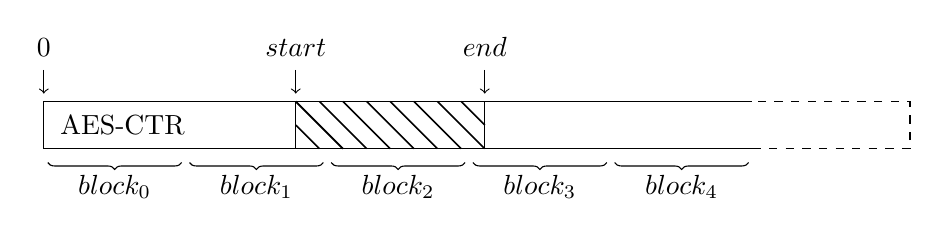
\begin{tikzpicture}
        \def\one{0.6}
        \def\width{9}
        \def\arrowstart{3.2}
        \def\arrowend{5.6}
        \def\padding{0.1}
        \def\arrowHeight{1}
        \def\dashLength{2}

        \draw (\width,0) -- (0,0) -- (0, \one) -- (\width,\one);
        \draw [dashed] (\width,0) -- (\width+\dashLength,0) -- (\width+\dashLength,\one) -- (\width,\one);

        \draw (1,\one/2) node {AES-CTR};

        \foreach \offset\name in{0/0,\arrowstart/$start$,\arrowend/$end$} {
                \begin{scope}[shift={(\offset,0)}]
                    \draw[->] (0,\arrowHeight) -- (0,\one+\padding)  node[above=10pt] {\name};
                    \draw (0,0) -- (0,\one);
                \end{scope}
            }

        \begin{scope}[shift={(\arrowstart,0)}]
            \def\a{2.4}
            \def\diff{1.8}
            \def\b{\one}
            \def\lw{0.2}

            \foreach \x [count=\i] in{0,0.3,0.6,...,\b}{
                    \draw [line width=\lw mm](\x,0)--(0,\x) (\a-\b+\x,\b)--(\a,\x);
                }
            \foreach \x [count=\i] in{0,0.3,0.6,...,\diff}{
                    \draw [line width=\lw mm](\x+\b,0)--(\x,\b);
                }
        \end{scope}

        \def\blockWidth{1.8}
        \foreach \i in{0,1,...,4} {
                \draw[decoration={brace,raise=5pt,mirror},decorate] (\i*\blockWidth+0.05,0) -- (\i*\blockWidth+\blockWidth-0.05,0) node[midway,below=6pt] {$block_{\i}$};
            }

    \end{tikzpicture}
    \caption{Pseudorandomness generator used within the HOPR protocol}
\end{figure}
